Dippy is the primarily the ``glue'' between two different technologies: PuLP and DIP.

PuLP~\cite{pulp} is a mathematical modelling language and toolkit that uses Python.
Users can define \ac{MILP} problems and solve them using a variety of solvers including CPLEX, Gurobi and CBC.
PuLP's solver interface is modular and thus can be easily extended to use other solvers such as \ac{DIP}.
For more details on PuLP see the PuLP project in the COIN-OR repository~\cite{coin_or}.

\acf{DIP}~\cite{decomp04} provides a framework for solving \ac{MILP} problems using 3 different methods\footnote{The skeleton for a fourth method (branch, relax and cut) exists in \ac{DIP}, but this method is not yet implemented.}:
\begin{enumerate}
	\item ``branch-and-cut'',
	\item ``branch-price-and-cut'',
	\item ``decompose-and-cut''.
\end{enumerate}
In this paper we will restrict our attention to branch-and-cut and branch-price-and-cut.

Branch-and-cut uses the classic branch-and-bound approach for solving \ac{MILP}s combined with the cutting plane method for removing fractionality encountered at the branch-and-bound nodes.
This framework is the basis of many state-of-the-art \ac{MILP} solvers including Gurobi and CBC.
\ac{DIP} provides callback functions that allow users to customise the solution process by adding their own cuts and running heuristics at each node.

Branch-price-and-cut uses Dantzig-Wolfe decomposition to split a large \ac{MILP} problem into a master problem and one or more subproblems.
The subproblems solve a pricing problem, defined using the master problem dual values, to add new variables to the master problem.
Branch-and-cut is then used on the master problem.

The cut generation and heuristic callback functions mentioned previously can also be used for branch-price-and-cut.
Extra callback functions enable the user to define their own routines for finding initial variables to include in the master problem and for solving the subproblems to generate new master problem variables.
For details on the methods and callback functions provided by \ac{DIP} see~\cite{decomp04}.

In addition to the \ac{DIP} callback functions (see \sbsref{sbs:callbacks}), we modified DIP to add another callback function that enables user-defined branching in \ac{DIP} and so can be used in any of the solution methods within \ac{DIP}.

\subsection{Callback Functions} \label{sbs:callbacks}

\begin{sloppypar}\paragraph{Advanced Branching}
We replaced \lstinline{chooseBranchVar} in the \ac{DIP} source with a new function \lstinline{chooseBranchSet}. 
This is a significant change to branching in DIP that makes it possible for the user to define:
\begin{itemize}
\item a {\it down} set of variables with (lower and upper) bounds that will be enforced in the down node of the branch; and,
\item an {\it up} set of variables with bounds that will be enforced in the up node of the branch.
\end{itemize}
A typical variable branch on an integer variable $x$ with integer bounds $l$ and $u$ and fractional value $\alpha$ can be implemented by:
\begin{enumerate}
\item choosing the down set to be $\{ x \}$ with bounds $l$ and $\lfloor \alpha \rfloor$;
\item choosing the up set to be $\{ x \}$ with bounds of $\lceil \alpha \rceil$ and $u$.
\end{enumerate}
However, other branching methods may use advanced branching techniques such as the one demonstrated in \sbsref{sbs:branch}.
From \ac{DIP}, \lstinline{chooseBranchSet} calls \lstinline{branch_method} in Dippy.\end{sloppypar}

\begin{sloppypar}\paragraph{Customised Cuts} % sloppypar deals with the line break issue by doing what you'd expect - pushing it to next line, bigger gaps
We modified \lstinline{generateCuts} (in the \ac{DIP} source) to call \lstinline{generate_cuts} in Dippy.
This enables the user to examine a solution and generate any customised cuts as necessary.
We also modified \lstinline{APPisUserFeasible} to call \lstinline{is_solution_feasible} in Dippy, enabling users to check solutions for feasibility with respect to customised cuts.\end{sloppypar}

\begin{sloppypar}\paragraph{Customised Columns (Solutions to Subproblems)}
We modified the \ac{DIP} function \lstinline{solveRelaxed} to call \lstinline{relaxed_solver} in Dippy.
This enables the user to utilise the master problem dual variables to produce solutions to subproblems (and so add columns to the master problem) using customised methods.
We also modified \lstinline{generateInitVars} to call \lstinline{init_vars} in Dippy, enabling users to customise the generation of initial columns for the master problem.\end{sloppypar}

\begin{sloppypar}\paragraph{Heuristics}
We modified \lstinline{APPheuristics} (\ac{DIP}) to call \lstinline{heuristics} (Dippy).
This enables the user to define customised heuristics at each node in the branch-and-bound tree (including the root node).\end{sloppypar}

\subsection{Interface}

The interface between Dippy (in Python) and DIP (in C++) is summarised in \figref{fig:interface}.
\begin{figure}[htp]
%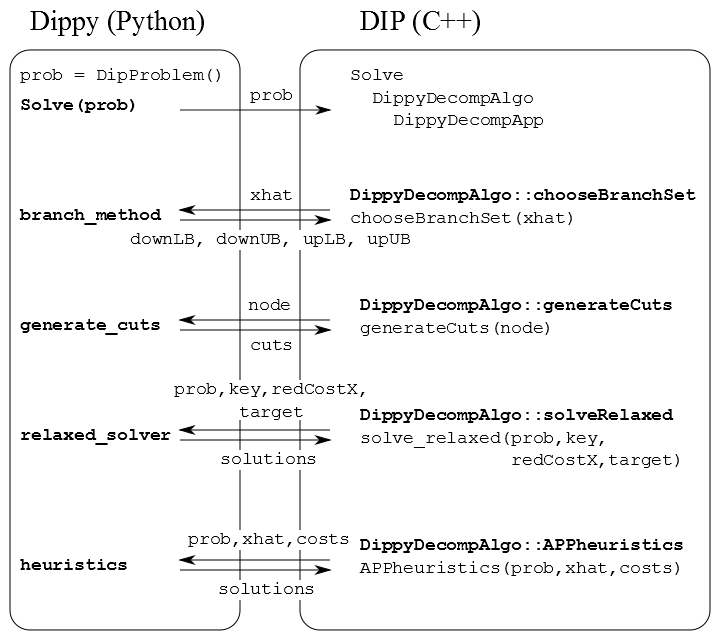
\includegraphics[bb=0 0 960 720,scale=0.45]{img/interface.png}
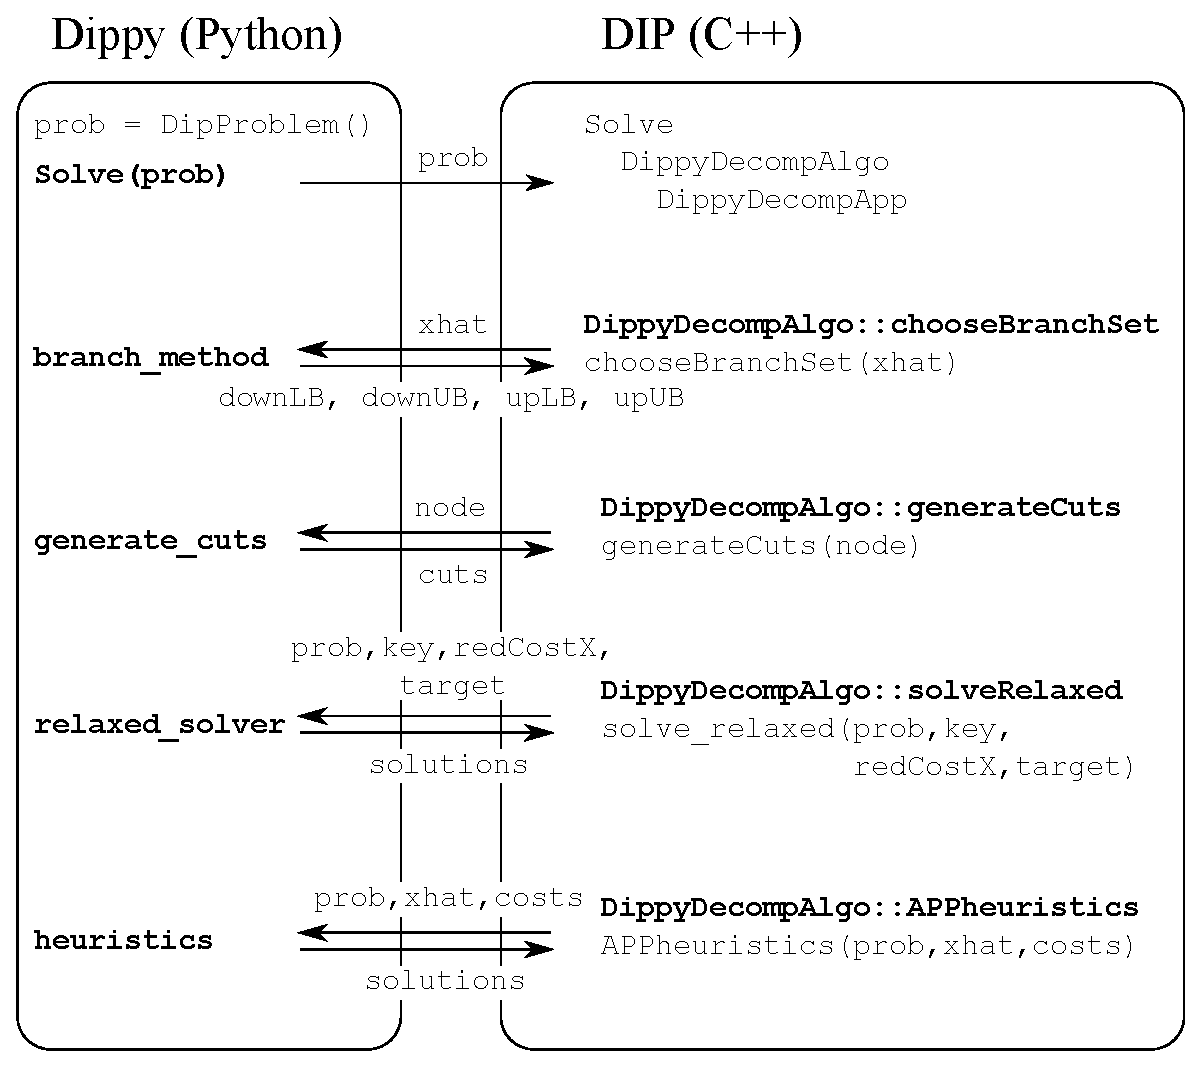
\includegraphics[scale=0.70]{img/diagram.eps}
\caption{Key components of interface between Dippy and DIP.} \label{fig:interface}
\end{figure}

\begin{sloppypar}The \ac{MILP} is defined as a \lstinline{DipProblem} and then solved using the \lstinline{Solve} command in Dippy, that passes the Python \lstinline{DipProblem} object, \lstinline{prob}, to DIP in C++.
\ac{DIP} \lstinline{Solve} creates a \lstinline{DippyDecompAlgo} object that contains a \lstinline{DippyDecompApp} object, both of which are populated by data from \lstinline{prob}.
As \ac{DIP} \lstinline{Solve} proceeds branches are created by the \lstinline{DippyDecompAlgo} object using \lstinline{chooseBranchSet} which passes the current node's fractional solution \lstinline{xhat} back to the \lstinline{branch_method} function in the \lstinline{DipProblem} object \lstinline{prob}.
This function generates lower and upper bounds for the ``down'' and ``up'' branches and returns to \lstinline{DippyDecompAlgo::chooseBranchSet}.
When \ac{DIP} generates cuts, it uses the \lstinline{DippyDecompApp} object's \lstinline{generateCuts} function which passes the current node \lstinline{node} to the \lstinline{DipProblem} object's \lstinline{generate_cuts} function.
This function generates any customised cuts and returns a list, \lstinline{cuts}, back to \lstinline{DippyDecompApp::generateCuts}.
These interfaces are replicated for the other callback functions provided by Dippy.\end{sloppypar}
